\chapter{Background}
\label{chapter:background}

This chapter will provide background on the major neural network architectures that are utilized in this research, as well as summarize and discuss research related to artificial intelligence-based \ac{T1D} management systems. Two of the most common \ac{T1D} management systems are \ac{BGL} prediction systems and insulin recommendation systems. Research into improving the accuracy and reliability of these systems could have a significant positive impact on the lives of those with \ac{T1D}. These systems can give people with \ac{T1D} more confidence in their decisions about how much insulin they should take and provide insight into how these decisions will affect their \ac{BGLs} over the following hours. As artificial intelligence and machine learning algorithms continue to evolve and improve, so too can the performance of these \ac{T1D} management systems.

\section{Time Series Prediction Models}
\label{section:time_series}

Neural networks are powerful machine learning models capable of learning to perform a wide variety of tasks across many domains given sufficient training data. In this research, the goal is to create neural network models capable of performing time series forecasting, where the task consists of predicting a future point in a time series given previous data from the series. However, due to the temporal nature of the data, a generic fully connected neural network will have difficulty processing time series data. As described in the following sections, \ac{RNNs} and Deep Residual Networks are two types of networks that are capable of processing and learning from such data.

\subsection{Recurrent Neural Networks}
\label{section:rnn}

\begin{figure*}[t]
    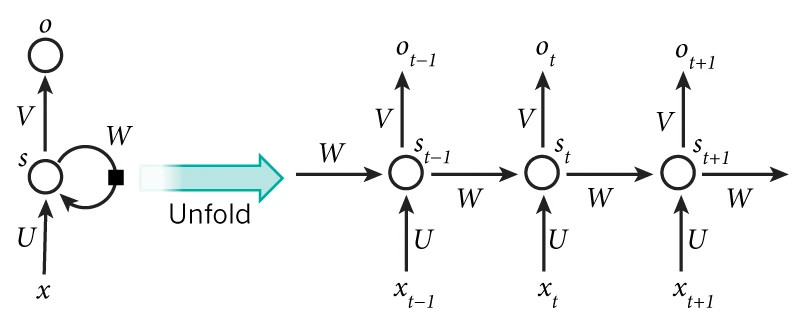
\includegraphics[width=\textwidth]{rnn}
    \caption{A visualization of an RNN \cite{lecun2015deep}.}
    \label{fig:rnn}
\end{figure*}

\ac{RNNs} are neural networks capable of learning from time series data. \ac{RNNs} process time series data in discrete time-steps, rather than processing all of it at once like a fully connected network would. \ac{RNNs} have three sets of weights, $W$, $U$, and $V$, that are used to compute a hidden state, $\text{{\bf s}}_{t}$ and an output $\text{{\bf o}}_t$ for every time step $t$. The state contains values that the network has recursively computed based on inputs from all previous time-steps. Along with the hidden state of the previous time-step, $\text{{\bf s}}_{t-1}$, the input at the current step in the time series, $\text{{\bf x}}_t$, is used to calculate both the output of the cell and the hidden state values. The hidden state at time $t$, $\text{{\bf s}}_t$, is calculated by the following formula:

\begin{center}
   $\text{{\bf s}}_t = f(W\text{{\bf s}}_{t-1} + U\text{{\bf x}}_{t} + \text{{\bf b}}_s)$
\end{center}
where $\text{{\bf b}}_s$ is a bias vector, and $f$ is a non-linear activation function. The tanh function or the sigmoid function are common choices for $f$. The output of the network at time $t$, $\text{{\bf o}}_t$, is calculated as follows:

\begin{center}
    $\text{{\bf o}}_t = f(V\text{{\bf s}}_{t} + \text{{\bf b}}_o)$
\end{center}
where $f$ is again a non-linear activation function and $\text{{\bf b}}_o$ is a different bias vector. Note that $f$ does not need to be the same in both equations. The weight matrices $W$, $U$, $V$, are learned via the Backpropagation Through Time (BPTT) algorithm \cite{werbos:bptt}. While \ac{RNNs} are capable of learning from time series data, they can have difficulty learning long distance dependencies due to the vanishing gradient problem \cite{bengio:vanishing}. The vanishing gradient problem refers to norm of the gradient rapidly shrinking to 0 for long-term dependencies during training, which makes it very difficult for \ac{RNNs} to learn the relationships between events that are temporally distant \cite{pascanu2013difficulty}. While there have been several proposed \ac{RNN} modifications that aim to remedy this issue, one of the most widely used is the \ac{LSTM} network \cite{hochreiter:nc97}.

\subsubsection{Long Short-Term Memory}
\label{section:lstm_background}

\begin{figure*}[t]
    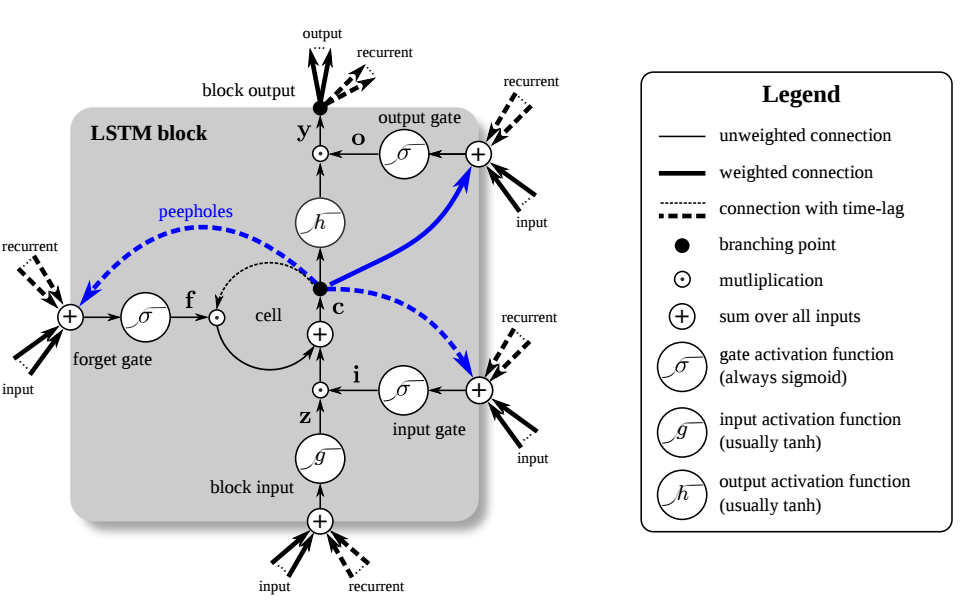
\includegraphics[width=\textwidth]{lstm}
    \caption{A diagram of an LSTM cell. The peephole connections represented by the blue lines are not part of the original LSTM architecture. Image from \cite{greff2016lstm} was slightly modified.}
    \label{fig:lstm}
\end{figure*}

In 1997, \ac{LSTM} networks were introduced as a solution to the vanishing gradient problem \cite{hochreiter:nc97}. \ac{LSTM} networks use multiplicative gates on the input and output for each cell. The purpose of the input gate is to prevent the information that has already been learned from the sequence to be perturbed by input events that are not relevant. Similarly, the output gate prevents irrelevant information from negatively affecting the output of a particular cell. In addition to gating the inputs and outputs of a cell, \ac{LSTM} cells also include a forget gate, which allows the cell to determine how much of the information captured in the previous hidden state should be remembered or forgotten \cite{gers1999learning}. These three gates allow the network to learn how much the previous hidden state and the input should affect the internal state of the cell, as well as how much of the internal state should be used when determining the output of the cell.

The values of the three gates at time $t$ are calculated by the following formulas:
\begin{center}
    $\text{{\bf f}}_t = \sigma(W^{(f)}\text{{\bf s}}_{t-1} + U^{(f)}\text{{\bf x}}_{t} + \text{{\bf b}}^{(f)})$\\
    $\text{{\bf i}}_t = \sigma(W^{(i)}\text{{\bf s}}_{t-1} + U^{(i)}\text{{\bf x}}_{t} + \text{{\bf b}}^{(i)})$\\
    $\text{{\bf o}}_t = \sigma(W^{(o)}\text{{\bf s}}_{t-1} + U^{(o)}\text{{\bf x}}_{t} + \text{{\bf b}}^{(o)})$\\
\end{center}

In these formulas, $\text{{\bf f}}_t$, $\text{{\bf i}}_t$, and $\text{{\bf o}}_t$ represents the values of the forget gate, input gate, and output gate at time $t$, respectively. The $\sigma$ in these formulas represents the sigmoid function. Once these gate values have been calculated, the output of the cell, $\text{{\bf z}}_t$ and the values of the internal state, $\text{{\bf c}}_t$ are calculated as follows:

\begin{center}
    $\text{{\bf z}}_t = \text{tanh}(W^{(z)}\text{{\bf s}}_{t-1} + U^{(z)}\text{{\bf x}}_{t} + b^{(z)})$\\
    $\text{{\bf c}}_t = \text{{\bf f}}_{t}\circ\text{{\bf c}}_{t-1} + \text{{\bf i}}_{t}\circ\text{{\bf z}}_t$
\end{center}

Finally, once the internal state $\text{{\bf c}}_t$ has been calculated, the version of the hidden state the will be used as input for the next cell, $\text{{\bf s}}_t$, can be calculated as follows:

\begin{center}
    $\text{{\bf s}}_t = \text{{\bf o}}_{t}\circ\text{tanh}(\text{{\bf c}}_t)$
\end{center}

This improved logic allows \ac{LSTM} networks to not only learn from time series data, but also learn what information should be remembered, and what can safely be forgotten. The element-wise multiplication of the forget gate with the previous value of the cell provides a path for the gradient to pass to previous cell states without being repeatedly diminished. This represents an elegant and powerful solution to the vanishing gradient problem and as such seen widespread adoption for time series prediction tasks.

\subsection{Deep Residual Networks}

Research on the generalization performance of neural networks has demonstrated that increasing the depth of a network often results in improved performance \cite{szegedy2015going, krizhevsky2012imagenet}. However, simply stacking a large number of layers in a network is not an infallible solution to improving its performance. Increasing the depth of a network not only increases the computational cost of training it but can also increase the difficulty of training \cite{glorot2010understanding}. One solution to this problem are shortcut (also called residual) connections, which skip at least one layer in a network. In \cite{he2016deep}, it was shown that using shortcut connections to simply add the original input of a stack of layers to that stack's output and pass that as input to the next stack allowed for very deep networks to achieve great performance on image recognition tasks \cite{he2016deep, Huang_2017_CVPR, he2016identity}. Additionally, the inclusion of these shortcut connections made the networks easier to train. These types of networks are known as residual networks, or ResNets. Very recent work has shown that deep residual networks can also achieve state-of-the-art performance on the task of time series forecasting, even without the aid of \ac{RNNs} \cite{oreshkin:nbeats}.

\subsubsection{N-BEATS}
\label{section:nbeats_background}

\begin{figure*}[t]
    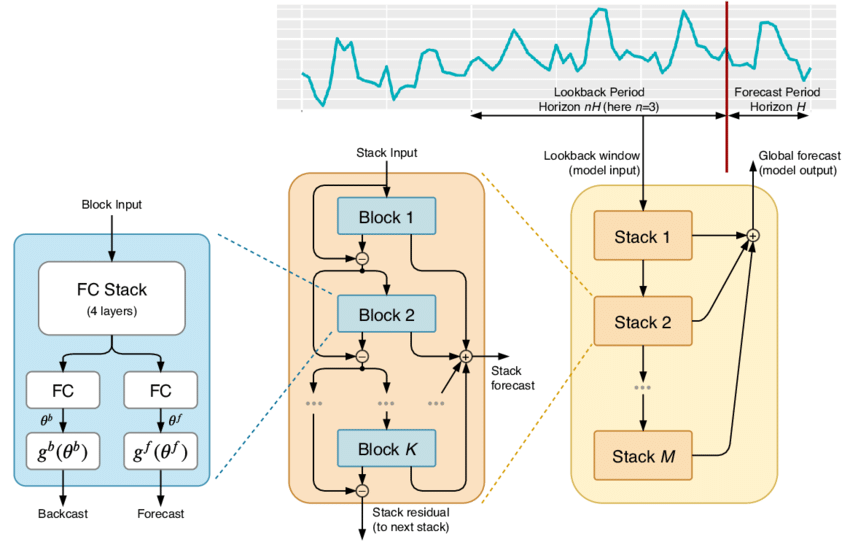
\includegraphics[width=\textwidth]{nbeats}
    \caption{A diagram of the original N-BEATS architecture \cite{oreshkin:nbeats}.}
    \label{fig:nbeats-background}
\end{figure*}

%The recently proposed architecture known as N-BEATS \cite{oreshkin:nbeats} has been shown to achieve state-of-the-art performance on many widely used time series datasets. The N-BEATS architecture is composed of basic blocks (neural networks) that are stacked in a doubly residual manner.

Oreshkin et al. have recently introduced a new architecture for time series forecasting, the \ac{N-BEATS}\cite{oreshkin:nbeats}. The \ac{N-BEATS} architecture is a deep residual model consisting of basic blocks that are stacked in a doubly residual manner. The basic building block of \ac{N-BEATS} is a fully connected structure that initially takes as input a fixed-size lookback period of past values of the target variable and outputs both forecast (estimates of future values) and backcast (estimates of past values) vectors. Blocks are organized into stacks such that the backcast of the current block is subtracted from its input and fed as input to the next block, whereas the forecast vectors from each block are summed up to provide the overall stack forecast. The stacks themselves are chained in a pipeline where the backcast output of one stack is used as input for the next stack. The overall model forecast is then computed by accumulating the forecasts across all the stacks. The \ac{N-BEATS} architecture has been shown to achieve state-of-the-art performance on a variety of widely used time series forecasting datasets \cite{oreshkin:nbeats}. % As such, the \ac{N-BEATS} architecture is a good choice for time series forecasting tasks.

\section{Blood Glucose Prediction}

Providing people with \ac{T1D} the ability to accurately anticipate their impending \ac{BGLs} would be an incredibly helpful and potentially life changing breakthrough. There has been much research with the goal of making this ambition closer to reality with artificial intelligence, specifically machine learning \cite{bunescu:svr_bgl,mirshekarian:bgl_pred,rubin_falcone:nbeats_bgl}. While the end goal of the research in this thesis is not to predict future \ac{BGLs}, there are many parallels between \ac{BGL} prediction and meal and bolus recommendation. \ac{BGL} prediction is essentially the converse of meal or bolus recommendation. \ac{BGL} prediction systems attempt to forecast a \ac{BGL} in the future given information in the present, while meal or bolus recommendation systems use the desired future \ac{BGL} (among other factors) given by the user to recommend a meal or bolus to take in the present in order to reach that \ac{BGL} target. As such, it is important to understand both sides of this problem.

The performance of \ac{BGL} prediction systems has improved due to advances in machine learning, and more specifically deep learning. Neural networks have allowed researchers to bypass the need for expensive, hand-engineered features. Advances in deep learning such as \ac{LSTM} networks \cite{hochreiter:nc97} and the \ac{N-BEATS} architecture \cite{oreshkin:nbeats} have specifically helped improve performance of such systems due to their ability to process temporal \ac{BGL} data. It is important to understand what types of techniques have led to improvement in \ac{BGL} prediction systems, as these same techniques will likely lead to a high level of performance in meal and bolus recommendation systems given the close relationship between the problems.

% Machine learning has been a catalyst in improving the accuracy of \ac{BGL} prediction systems.
In \cite{bunescu:svr_bgl}, a support vector regression model was trained on hand-engineered physiological features based on the raw features extracted from real patient data. This machine learning based approach was shown to outperform three physicians at predicting \ac{BGLs} 30 and 60 minutes into the future. However, creating these hand-engineered features can be time-consuming, expensive, and require the aid of experts in the field of \ac{T1D}. Using deep learning models such as neural networks can eliminate the need for hand-engineered features, as these models can learn relevant features automatically.

In \cite{mirshekarian:bgl_pred}, the authors create a neural network model utilizing the \ac{LSTM} networks described in Section~\ref{section:lstm_background} to predict future \ac{BGLs}. To make these predictions, the models use only raw features from the data, such as a recent history of \ac{BGLs}, insulin, and the carbohydrate counts from recent meals. One of the three training scenarios the authors outlined in the paper, the "what-if" scenario, is a particularly interesting scenario due to its relationship with the meal and bolus recommendation problems. In this scenario, the \ac{BGL} is predicted with the aid of "what-if" events, specifically meals and bolus that occur after the current time, but before the end of the prediction window (the current time + 30 or 60 minutes). 
% Since the models are trained on retroactive data that had already been collected, it is possible to use data from future events to help make the prediction. 
This scenario is useful as it is essentially predicting \ac{BGLs} given some future action intended by the user, such as how many carbs will be in a meal that they plan to eat soon, or how much insulin they plan to bolus in the new few minutes. This could provide people with \ac{T1D} an estimate as to how much a meal or bolus will affect their \ac{BGL} before taking the action. This is essentially the inverse of the research in this thesis, where instead of answering the question "What would my \ac{BGL} be if I eat or bolus this much?", this research aims to answer the question "How much do I need to eat or bolus to get my \ac{BG} to this level?".

%Neural networks are flexible and robust machine learning algorithms that can learn representations of data automatically. Recurrent neural networks have long been the de facto method for processing time-series data in deep learning models. This has been especially true since 1997, when LSTMs were first introduced as a solution to the vanishing gradient problem \cite{hochreiter:nc97}. However, a recently proposed architecture known as N-BEATS \cite{oreshkin:nbeats} has been shown to achieve state-of-the-art performance on many widely used time-series datasets. The N-BEATS architecture, composed of basic blocks (neural networks) that are stacked in a doubly residual manner, has been proven to perform very well on the task of BGL prediction given a few modifications. 

Given the state-of-the-art performance of the \ac{N-BEATS} architecture for time series forecasting tasks Section~\ref{section:nbeats_background}, it is also a natural choice for the \ac{BGL} prediction task. The authors of \cite{rubin_falcone:nbeats_bgl} proposed three important modifications to the original \ac{N-BEATS} architecture to make it better suited for this task. The first, and potentially the most important of these modifications, was the introduction of an \ac{LSTM} into each block to help account for the temporal nature of the blood glucose data. The second proposed modification was the inclusion of additional time series variables, specifically recent carb counts and bolus doses, for each block as context. Without this information, the model would not be able to learn the effects that carbs and insulin have on a subject’s \ac{BGLs}, which would be a missed opportunity for improvement. Finally, the third proposed modification was restructuring the loss function to aid each block in a stack to learn better intermediate representations. With these improvements, the authors achieved top performance on the task of \ac{BGL} prediction \cite{kdh-2020-proceedings}



\section{Insulin Recommendation Systems}

Providing people with \ac{T1D} the ability to preview their future \ac{BGLs} would be of great help in improving the management of their BGLs. However, without the tools to inform a user how to correct their \ac{BGL} if they are predicted to rise too high or sink too low, the usefulness of \ac{BGL} prediction systems is fairly limited. Insulin recommendation systems provide the user with recommendations for how much insulin they should take to lower their \ac{BGL} to the desired target in the near future. There have been a wide range of AI techniques employed to make these insulin recommendation systems such as case-based reasoning \cite{pesl:case_based}, K-nearest-neighbors methods \cite{tyler:knn}, and neural networks \cite{zhu:bolus_drl}. Accuracy is paramount with insulin recommendation systems, as recommendations that are too high or too low can lead to hypoglycemia or hyperglycemia, respectively. Both can cause several long-term complications if not hastily corrected. Therefore, it is critical that insulin recommendation systems be as accurate as possible.

The bolus recommendation system introduced in \cite{pesl:case_based} uses case-based reasoning to provide recommendations for the parameters to be used by a bolus calculator. In this system, cases consist of the meal scenario, the solution (the recommended bolus calculator parameters), and the outcome (the postprandial glucose excursion). When making a recommendation, the system searches through past cases to find a case that is similar to the current situation. If one such case is found, the bolus parameters used in the past case are recommended. If these parameters do not produce the desired outcome (i.e., the subjects postprandial glucose excursion is too high or too low) the original case’s solution is revised by an expert. If no cases similar to the current case are found, a new case is created. This case-based reasoning approach allows the creation of a bolus recommendation system completely personalized to a specific person with \ac{T1D}. However, this system is not learning how meals or boluses affect a person’s \ac{BGL}. It is recalling the bolus recommendations from past instances of similar situations, which have been revised by a clinical expert. While this can lead to very accurate and safe bolus recommendations, it requires an expert to look over the cases and revise the recommendations by hand on a regular basis. This is an expensive and time-consuming task. This also means that when a unique meal scenario that has not been seen before is encountered, the system lacks the ability to make an intelligent prediction.

The authors of \cite{tyler:knn} introduce an insulin recommendation system that provides a user with recommendations on how to improve their \ac{BGLs} through adjustments in their insulin routines. This system uses the K-nearest-neighbors machine learning algorithm to provide up to four (out of 12 possible options) weekly recommendations for adjustments to a user’s insulin dosages. This is done by looking at \ac{BGL}, insulin, and physical activity from the user and classifying which types of recommendations they could benefit from. The goal of this system is to maximize the amount of time that a user spends with a \ac{BGL} in a healthy range while minimizing the amount of time spent in the hypoglycemic range. The system may recommend the user to adjust factors such as their basal insulin rate, their carbs-to-insulin ratio, or their correction factor. While this system offers multiple different types of recommendations, they are adjustments that will have a positive effect on a subject’s \ac{BGL} in a longer-term. As such, it is not as flexible or dynamic as a system that can provide a user with recommendations for real time bolus dosages.

The work in \cite{cappon:bolus_nn} shows that deep learning can be used to personalize the calculation of bolus doses. The authors demonstrated that using a simple feed-forward neural network to calculate bolus doses can outperform other modern methods for \ac{CGM}-based personalized bolus calculators. Neural network models can make recommendations that are specific to an individual by not only considering factors such as insulin on board and target \ac{BGLs}, but also subject-specific parameters such as body weight and insulin sensitivity. While this work shows the usefulness of neural networks for personalizing an individual’s bolus recommendations, this approach does not consider any previous history of \ac{BGLs}, meals, or boluses. Using these features could potentially allow a bolus advisor to make recommendations that are not only personalized for an individual but are personalized for an individual in a specific situation. This would likely result in even better recommendations.

In \cite{zhu:bolus_drl}, the authors proposed a deep reinforcement learning based system for recommending bolus dosages for people with \ac{T1D}. The general approach was to take an action (deliver a bolus) at the time of the meal given the state of the environment (values of various sensors in a glucose control systems) that would maximize the amount of time that a subject’s \ac{BGL} stayed in a healthy range while simultaneously minimizing the amount of time spent in the hypoglycemia range. Since the authors opted to use a reinforcement learning approach, they need an environment in which the models can repeatedly explore various bolus dosages in order to learn a bolus recommendation policy. The ideal environment would be provided by real individuals with \ac{T1D}. However, this would be incredibly unsafe. Even with safety constraints in place, a bad recommendation could force a subject's \ac{BGLs} into a hypoglycemic state. Since training on human subjects is infeasible, the authors used a simulator to train their model, namely the UVA/Padova simulator \cite{dalla_man:simulator}. While simulated data is a more appropriate choice in this situation, it is unclear how well the learned policy would work on data from a real human subject.

The use of insulin recommendation systems can assist people with \ac{T1D} with managing their \ac{BGLs}. There are many different approaches and techniques being used to developing these systems. Similar to \ac{BGL} prediction systems, advances in artificial intelligence continue to enable the creation of improved systems for insulin recommendations. These systems may eventually allow for people with \ac{T1D} to avoid hypoglycemia or hyperglycemia through accurate, safe, and reliable insulin recommendations.

%\section{Contribution}

%The contribution of this thesis is a general neural network architecture that can be trained to make bolus recommendations and meal recommendations. Two architectures were developed and compared on the tasks of bolus and carbohydrate recommendations, an LSTM-based architecture and an N-BEATS-based architecture. The LSTM-based architecture draws inspiration from the architecture introduced in \cite{mirshekarian:bgl_pred} for the task of BGL prediction. The architecture was redesigned to make meal or bolus recommendations using similar input data to that of the original BGL prediction system. The N-BEATS-based architecture is based on the original N-BEATS architecture \cite{oreshkin:nbeats}, and the modified version that was built for the task of BGL prediction \cite{rubin_falcone:nbeats_bgl}. Our N-BEATS-based architecture makes additions to these architectures which make them better suited for the tasks of bolus and meal recommendations. Both architectures are trained on the OhioT1DM dataset \cite{marling:ohiot1dm}, which contains data from real people with T1D. The goal of this research is to use real-patient data and proven BGL prediction architectures to create accurate, personalized bolus and meal recommendation systems.